\documentclass[14pt,a4paper,oneside]{extbook}
\usepackage[utf8]{vietnam}
\usepackage{amsmath,amssymb,mathrsfs,fancyhdr,enumerate,multirow,makecell}
\usepackage{tkz-euclide,tikz-3dplot,tikz,tkz-tab}
\usetikzlibrary{arrows.meta,calc,intersections,angles,quotes,backgrounds,shapes.geometric,patterns,through,shadows,positioning}
\usepackage{yhmath}
\usepackage[top=0.7cm, bottom=0.7cm, left=1.0cm, right=1.0cm, headheight=16pt, headsep=3mm, footskip=5mm]{geometry}
\usepackage[hidelinks,unicode]{hyperref}
\usepackage{qrcode}
\usepackage[many]{tcolorbox}
\usepackage{fontawesome}

\pagestyle{fancy}
\fancyhf{}
\fancyhead[L]{\footnotesize\bfseries\color{teal!85!black}\faBook~SỔ TAY KIẾN THỨC TOÁN 5}
\fancyhead[R]{\footnotesize\bfseries\color{blue!85!black}Lớp Toán Thầy Lĩnh -- loptoanthaylinh.vn}
\fancyfoot[C]{\footnotesize\bfseries\color{gray!80!black}-- Sổ tay kiến thức: Bài 49. Hình khai triển hình lập phương, hình hộp chữ nhật, hình trụ --}
\renewcommand{\headrulewidth}{0.4pt}

\begin{document}

% --- BANNER TIÊU ĐỀ BÀI HỌC ---
\noindent
\begin{tcolorbox}[
  enhanced,
  colback=teal!8!white,
  colframe=teal!80!black,
  arc=3mm,
  boxrule=1.1pt,
  width=\linewidth,
  halign=center,
  top=2.2mm, bottom=2.2mm,
  left=3mm, right=3mm,
  drop fuzzy shadow
]
  {\large\bfseries\color{teal!95!black}\faBookmark\ BÀI 49. HÌNH KHAI TRIỂN HÌNH KHỐI (HLP, HHCN, HÌNH TRỤ)}\\[2pt]
  {\scriptsize\color{black!75}\itshape Nhận biết các mặt đáy, mặt bên và cấu trúc hình khai triển phẳng trên 1 trang A4}
\end{tcolorbox}

\vspace{3.2mm}
% --- KHỐI 1: KHÁI NIỆM HÌNH KHAI TRIỂN ---
\noindent
\begin{minipage}[t]{0.56\textwidth}
  \begin{tcolorbox}[
    enhanced,
    title={\footnotesize\bfseries\color{white}\faCube\ 1. Khái niệm Hình khai triển},
    colback=blue!2!white,
    colframe=blue!75!black,
    arc=2.5mm, boxrule=0.8pt, top=1.8mm, bottom=1.8mm, left=2.2mm, right=2.2mm
  ]
    \footnotesize
    $\bullet$ Cắt theo các cạnh của một hình khối và trải phẳng trên mặt bàn $\rightarrow$ ta được \textbf{hình khai triển} của hình khối đó.\\
    $\bullet$ \textbf{Hình lập phương}: Khai triển gồm \textbf{6 hình vuông} bằng nhau.\\
    $\bullet$ \textbf{Hình hộp chữ nhật}: Gồm \textbf{6 hình chữ nhật}, tạo thành $3$ cặp mặt đối diện bằng nhau từng đôi một.\\
    $\bullet$ \textbf{Hình trụ}: Khai triển gồm \textbf{1 hình chữ nhật} (mặt xung quanh uốn cong) và \textbf{2 hình tròn} bằng nhau (hai đáy).
  \end{tcolorbox}
\end{minipage}%
\hfill
\begin{minipage}[t]{0.42\textwidth}
  \begin{tcolorbox}[
    enhanced,
    title={\footnotesize\bfseries\color{white}\faEye\ Mẫu khai triển chữ T},
    colback=teal!2!white,
    colframe=teal!75!black,
    arc=2.5mm, boxrule=0.8pt, top=1.8mm, bottom=1.8mm, left=1.5mm, right=1.5mm,
    halign=center
  ]
    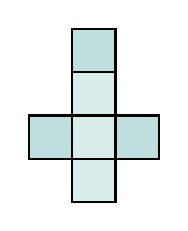
\begin{tikzpicture}[scale=0.55]
      \draw[thick, fill=teal!15] (1,0) rectangle (2,1);
      \draw[thick, fill=teal!25] (0,1) rectangle (1,2);
      \draw[thick, fill=teal!15] (1,1) rectangle (2,2);
      \draw[thick, fill=teal!25] (2,1) rectangle (3,2);
      \draw[thick, fill=teal!15] (1,2) rectangle (2,3);
      \draw[thick, fill=teal!25] (1,3) rectangle (2,4);
    \end{tikzpicture}\\[2pt]
    {\tiny\color{teal!95!black}\bfseries Gấp lại theo các mép sẽ được hình lập phương}
  \end{tcolorbox}
\end{minipage}

\vspace{3mm}

% --- KHỐI 2: ĐẶC ĐIỂM HÌNH TRỤ ---
\noindent
\begin{tcolorbox}[
  enhanced,
  title={\footnotesize\bfseries\color{white}\faCylinder\ 2. Khai triển đặc biệt của Hình trụ},
  colback=purple!2!white,
  colframe=purple!70!black,
  arc=2.5mm, boxrule=0.8pt, top=1.8mm, bottom=1.8mm, left=2.5mm, right=2.5mm
]
  \footnotesize
  Khi trải phẳng mặt xung quanh của hình trụ, ta được một hình chữ nhật có:\\
  $\bullet$ Một kích thước bằng \textbf{chiều cao} của hình trụ ($h$).\\
  $\bullet$ Kích thước còn lại bằng đúng \textbf{chu vi của hình tròn đáy}: $C = d \times 3,14 = 2 \times r \times 3,14$.\\
  $\bullet$ Hai đáy là hai hình tròn giống hệt nhau gắn ở hai phía đối diện.
\end{tcolorbox}

\vspace{3mm}

% --- KHỐI 3: SƠ ĐỒ TƯ DUY ---
\noindent
\begin{tcolorbox}[
  enhanced,
  title={\footnotesize\bfseries\color{white}\faSitemap\ Sơ đồ tư duy: Nhận dạng hình khai triển hợp lệ},
  colback=yellow!2!white,
  colframe=teal!85!black,
  arc=3mm, boxrule=0.9pt, top=1.8mm, bottom=1.8mm, left=1.5mm, right=1.5mm,
  halign=center
]
  \begin{tikzpicture}[
    scale=0.92,
    every node/.style={transform shape},
    b1/.style={rectangle, rounded corners=4pt, fill=blue!15, draw=blue!70!black, text=blue!90!black, font=\bfseries\scriptsize, inner sep=4pt, align=center},
    b2/.style={rectangle, rounded corners=4pt, fill=teal!15, draw=teal!70!black, text=teal!90!black, font=\bfseries\scriptsize, inner sep=4pt, align=center},
    b3/.style={rectangle, rounded corners=4pt, fill=green!15, draw=green!70!black, text=green!90!black, font=\bfseries\scriptsize, inner sep=4pt, align=center}
  ]
    \node[b1] (hlp) at (-5.8, 0) {HÌNH LẬP PHƯƠNG\\$6$ mặt vuông bằng nhau\\(Dạng 1-4-1, 2-3-1)};
    \node[b2] (hhcn) at (0, 0) {HÌNH HỘP CHỮ NHẬT\\$6$ mặt chữ nhật\\($3$ cặp đối bằng nhau)};
    \node[b3] (ht) at (5.8, 0) {HÌNH TRỤ\\$1$ HCN thân quấn quanh\\$2$ hình tròn đáy 2 phía};

    \draw[teal!85!black, thick, -{Stealth[length=2.5mm]}] (hlp) -- (hhcn);
    \draw[teal!85!black, thick, -{Stealth[length=2.5mm]}] (hhcn) -- (ht);
  \end{tikzpicture}
\end{tcolorbox}

\vspace{3mm}

% --- KHỐI 4: QUY TẮC CẶP MẶT ĐỐI & BẪY TRẮC NGHIỆM ---
\noindent
\begin{minipage}[t]{0.54\textwidth}
  \begin{tcolorbox}[
    enhanced,
    title={\footnotesize\bfseries\color{white}\faArrowsAltH\ Mẹo tìm hai mặt đối diện},
    colback=green!3!white,
    colframe=green!60!black,
    arc=2.5mm, boxrule=0.8pt, top=1.8mm, bottom=1.8mm, left=2.2mm, right=2.2mm
  ]
    \footnotesize
    Trên hình khai triển hình lập phương dạng dải hàng ngang:\\
    $\bullet$ Hai mặt \textbf{cách nhau 1 ô vuông} sẽ trở thành \textbf{hai mặt đối diện} khi gấp lại.\\
    $\bullet$ Hai mặt nằm về cùng một phía của dải không thể là hai đáy đối nhau.
  \end{tcolorbox}
\end{minipage}%
\hfill
\begin{minipage}[t]{0.44\textwidth}
  \begin{tcolorbox}[
    enhanced,
    title={\footnotesize\bfseries\color{white}\faExclamationTriangle\ Mẹo tránh bẫy trắc nghiệm},
    colback=red!2!white,
    colframe=red!70!black,
    arc=2.5mm, boxrule=0.8pt, top=1.8mm, bottom=1.8mm, left=2.2mm, right=2.2mm
  ]
    \footnotesize
    $\bullet$ Không phải cứ $6$ ô vuông dính nhau là gấp được thành hình lập phương (nếu có $4$ ô thành hình vuông $2 \times 2$ là \textbf{không gấp được})!\\
    $\bullet$ Hình trụ: $2$ đáy phải nằm ở \textbf{hai phía đối diện} của hình chữ nhật.
  \end{tcolorbox}
\end{minipage}

\end{document}
